\documentclass{article}
\usepackage{graphicx} % Required for inserting images
\usepackage[top=0.9in, bottom=1in, left=1.5in, right=1.5in]{geometry}
\usepackage[utf8]{inputenc}
\usepackage[icelandic]{babel}
\usepackage[T1]{fontenc}
\usepackage[sc]{mathpazo}
\usepackage[parfill]{parskip}
\renewcommand{\baselinestretch}{1.2}
% Tables and lists
\usepackage{booktabs,tabularx}
\usepackage{multirow}
\usepackage{enumerate}
\usepackage{adjustbox}
\usepackage{multicol}
\usepackage{xcolor}
\usepackage{algpseudocode}
\usepackage{algorithm}
\usepackage{tikz}
\usepackage{nicefrac}
\usepackage{changepage}
\usepackage{fancyvrb}
\usepackage{xlop}
\usepackage{hyperref}
\usepackage{pgfplots}
\pgfplotsset{compat=1.18}
\usetikzlibrary{arrows,arrows.meta, positioning, calc, graphs}

% Math
\usepackage{amsmath, amsfonts, amssymb, amsthm}
% Graphics

\usepackage{graphicx}
\usepackage{tikz}
% Code environment
\usepackage{minted}
%\usepackage{bm}
%\usepackage{siunitx}
%\usepackage{animate}
%\usepackage{hyperref}
%\usepackage{movie15}
%\usepackage{multicol}
%\usepackage{changepage}
\title{Tölvugrafík Heimadæmi 4}
\author{Ragnar Björn Ingvarsson, rbi3}
\tikzset{->, >=stealth', shorten >=1pt, node distance=2cm,thick, main node/.style={circle,draw,minimum size=3em}}


\begin{document}
\renewcommand\thepage{}
	
	\maketitle

	\newpage
	\setcounter{page}{1}
	\renewcommand\thepage{\arabic{page}}

	\section{}

	Snúningur og hliðrun geta verið víxlnar t.d. í tilvikinu þar sem hliðrað 
	og snúið er um sama ás, þ.e. þegar hliðrað er í x-ás og svo snúið um 
	x-ás.

	\[T_x = \begin{bmatrix} 
		1 & 0 & 0 & \delta \\ 
		0 & 1 & 0 & 0 \\ 
		0 & 0 & 1 & 0 \\ 
		0 & 0 & 0 & 1 
		\end{bmatrix}, R_x = 
		\begin{bmatrix}
		1 & 0 & 0 & 0 \\
		0 & cos(\theta) & -sin(\theta) & 0 \\
		0 & sin(\theta) & cos(\theta) & 0 \\
		0 & 0 & 0 & 1
		\end{bmatrix}\]
		\[T_x \cdot R_x =
		\begin{bmatrix}
		1 & 0 & 0 & \delta \\
		0 & cos(\theta) & -sin(\theta) & 0 \\
		0 & sin(\theta) & cos(\theta) & 0 \\
		0 & 0 & 0 & 1
		\end{bmatrix}, 
		R_x \cdot T_x =
		\begin{bmatrix}
		1 & 0 & 0 & \delta \\
		0 & cos(\theta) & -sin(\theta) & 0 \\
		0 & sin(\theta) & cos(\theta) & 0 \\
		0 & 0 & 0 & 1
		\end{bmatrix}\]

		\section{}


		\begin{itemize}
			\item[a)]
				Hér snúum við fyrst, svo húsið fer í annan fjórðung 
				hnitakerfisins og dettur á vinstri hlið sína, síðan færum 
				við það um (2,-1) og skölum svo um (1,2) svo húsið verður 
				breitt. Síðan færum við það aðeins í lokin.
				\begin{center}
		\begin{tikzpicture}
			\begin{axis}[
				cycle list name=black white,
				xmin=-1.9,xmax=1.9,ymin=0,ymax=4.9,
				xlabel=$x$,
				ylabel=$y$,
				grid=major,
				grid style={thin,densely dotted,black!30}]
				\addplot coordinates
					{(0,2) 
					(1,2) 
					(1,4) 
					(0,4) 
					(-1,3) 
					(0,2) 
					(0,4)};
			\end{axis}
		\end{tikzpicture}
	\end{center}
			\item[b)]
				Hér hins vegar hliðrum við aðeins fyrst og svo skölum við 
				um (1,2) áður en við snúum. Þetta veldur því að í stað þess 
				að húsið verði breitt þá verður það hátt. Síðan, eftir að 
				það er orðið hátt snúum við og það dettur aftur á vinstri 
				hlið sína.
		\begin{center}
		\begin{tikzpicture}
			\begin{axis}[
				cycle list name=black white,
				xmin=-3.9,xmax=1.9,ymin=0,ymax=3.9,
				xlabel=$x$,
				ylabel=$y$,
				grid=major,
				grid style={thin,densely dotted,black!30}]
				\addplot coordinates
					{(-1,2) 
					(1,2) 
					(1,3) 
					(-1,3) 
					(-3,2.5) 
					(-1,2) 
					(-1,3)};
			\end{axis}
		\end{tikzpicture}
	\end{center}
		\end{itemize}

		\section{}

		Við skulum halda þessu einföldu og nota fyrst hliðrun um 
		(-1.5, -0.5) til að koma kassanum í miðju hnitakerfisin, skalað 
		svo um (1.0, 2.0) áður en við snúum svo við þurfum ekki að gera 
		skölun í bæði x og y, svo getum við snúið um 45 gráður og loks hliðrað 
		um (2,2) til að koma honum á réttan stað.

		Þetta sameinast í samsetta vörpunarfylkið

		\[T_2 \cdot R \cdot S \cdot T_1 = \begin{bmatrix}
			\frac{\sqrt{2}}{2} & -\sqrt{2} & 0 & 2 - \frac{\sqrt{2}}{4} \\
			\frac{\sqrt{2}}{2} & \sqrt{2} & 0 & 2 - \frac{\nicefrac{5}{2}}{\sqrt{2}} \\
		0 & 0 & 1 & 0 \\
		0 & 0 & 0 & 1
		\end{bmatrix}\]

		\newpage
		\section{}

		\url{https://skogarbjorn.github.io/h4/billy/billy.html}
		\begin{center}
			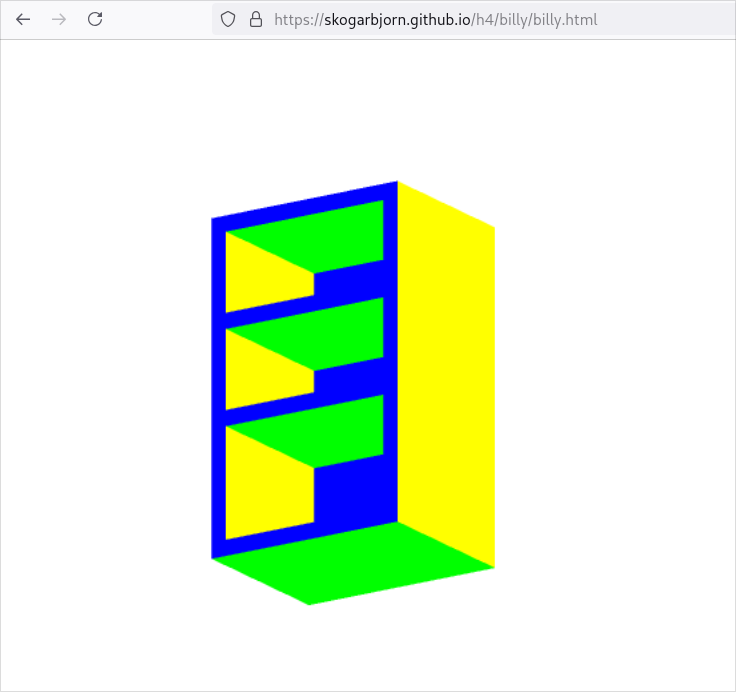
\includegraphics[scale=0.35]{billy.png}
		\end{center}

		\newpage
		\section{}

		\url{https://skogarbjorn.github.io/h4/time/time.html}
		\begin{center}
			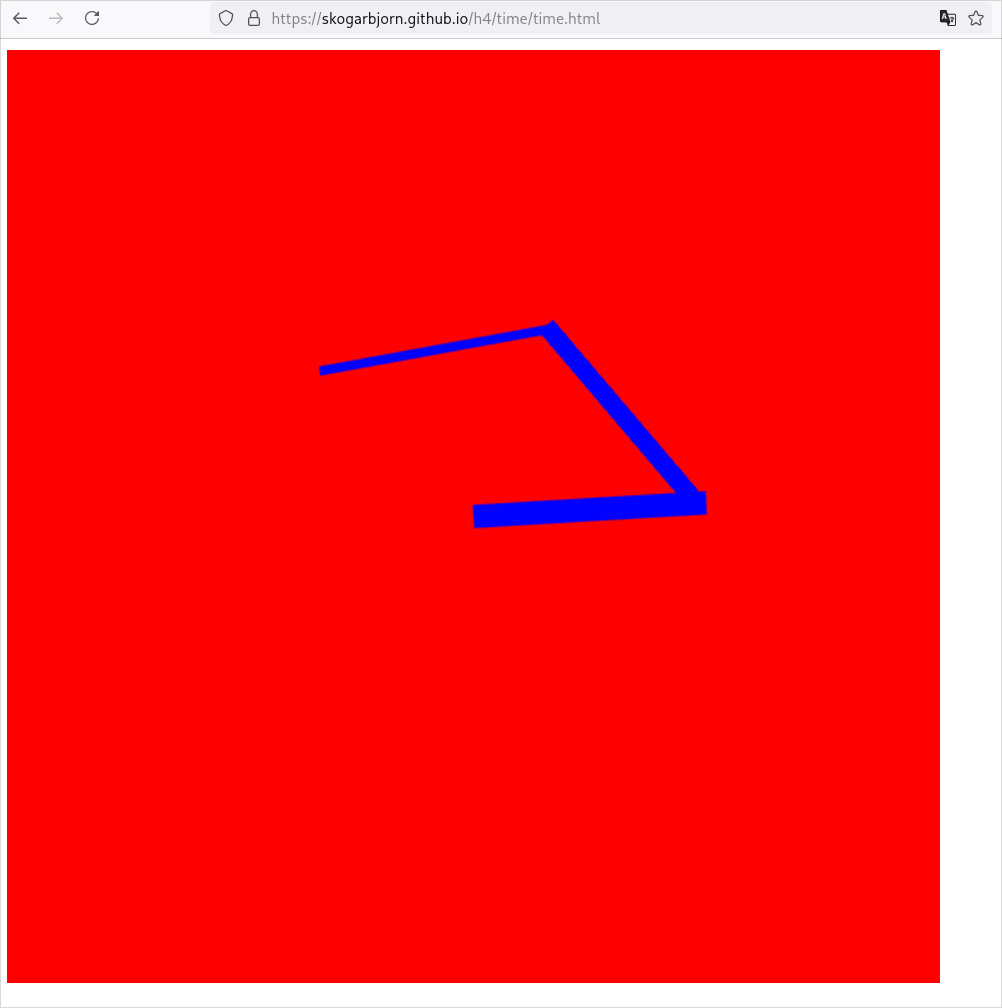
\includegraphics[scale=0.35]{time.png}
		\end{center}


\end{document}
